\section{Descripción estructural de un multiplexor con \textit{IP Catalog} \label{sec:s2}}

\begin{center}
	\begin{minipage}{12cm}
		\begin{tcolorbox}[title=Actividad 2]
			Describir el multiplexor en forma estructural usando una función creada por el \textit{IP Catalog} siguiendo los pasos descritos en el documento o presentación. Simular el multiplexor.
		\end{tcolorbox}	
	\end{minipage}
\end{center}

Para generar la instancia con \textit{IP Catalog}, que se va a utilizar en el módulo principal, se realizaron los siguientes pasos:

\begin{itemize}
	\item En el apartado de \textit{Library}, se seleccionó \textit{Basic Functions} $->$ \textit{Miscellaneous} $->$ \textit{LPM\_MUX} (Ver \autoref{fig:ipcatalog1}).
	\item Se coloco el nombre de la instancia, se seleccionó como archivo tipo Verilog y se dio clic en el botón \textit{OK} (Ver \autoref{fig:ipcatalog2}).
	\item Se indicó que el módulo debe tener 2 entradas, una salida y que no se iba a dividir en etapas, conocidas como \textit{pipelines} (Ver \autoref{fig:ipcatalog3}).
	\item Se dio clic en el botón \textit{Next} (Ver \autoref{fig:ipcatalog4}).
	\item Se seleccionaron las opciones para la creación de los archivos \textit{MyMux.cmp}, \textit{MyMux\_inst.v} y \textit{MyMux\_bb.v} (Ver \autoref{fig:ipcatalog5}).
	\item Finalmente, se dio clic en el botón \textit{Yes}, para instanciar el archivo en el proyecto (Ver \autoref{fig:ipcatalog6}).
\end{itemize}

Como se observa en la \autoref{fig:ipcatalog7} se generó la instancia del archivo en la carpeta del proyecto.

La visualización RTL del multiplexor, usando descripción estructural en Verilog, y con ayuda de \textit{IP Catalog}, se muestra en la \autoref{fig:mux_ipcatalog_rtl}. La implementación con la herramienta, anteriormente mencionada, hace la instanciación de varios módulos, vistos en la \autoref{fig:mux_ipcatalog_rtl2}, \autoref{fig:mux_ipcatalog_rtl3} y \autoref{fig:mux_ipcatalog_rtl4}. Las simulaciones se visualizan en la \autoref{fig:mux_ipcatalog_wave}, en donde se muestra que el multiplexor descrito opera de manera correcta.

En los Anexos se localiza la descripción en Verilog de este multiplexor. Debido a que se utilizó la herramienta \textit{IP Catalog}, el código solo tiene la descripción del módulo de más alta jerarquía, en donde se realiza la declaración de las entradas y la salida, para luego instanciar al módulo llamado ``MyMux'' con la etiqueta ``u0''. Cabe señalar que los argumentos de la instancia se deben colocar en el orden correcto.

\begin{figure}[ht]
	\centering
	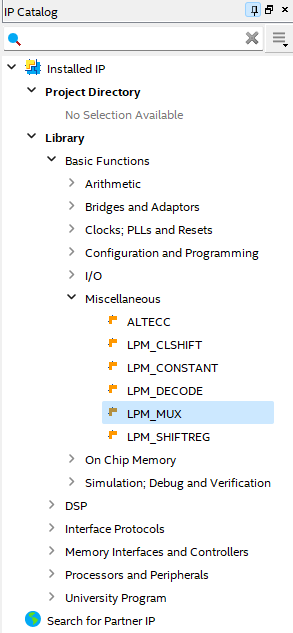
\includegraphics[scale=0.69]{IPCatalog1.png}
	\caption{Instanciación del multiplexor con \textit{IP Catalog} (Paso 1). \label{fig:ipcatalog1}}
\end{figure}

\begin{figure}[ht]
	\centering
	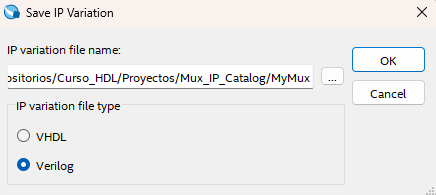
\includegraphics[scale=0.69]{IPCatalog2.png}
	\caption{Instanciación del multiplexor con \textit{IP Catalog} (Paso 2). \label{fig:ipcatalog2}}
\end{figure}

\begin{figure}[ht]
	\centering
	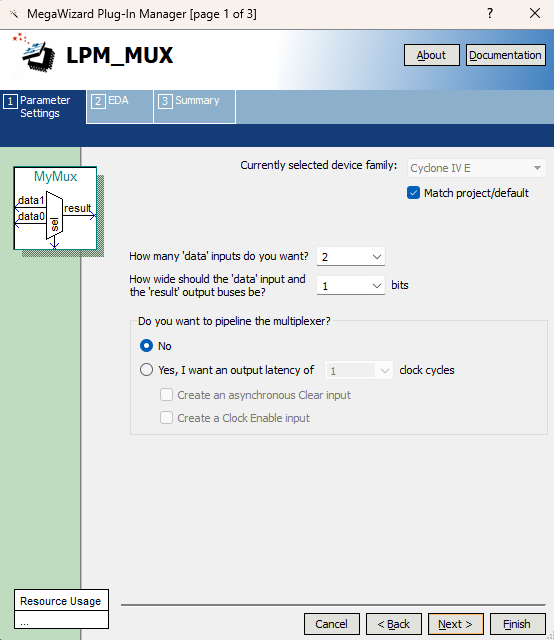
\includegraphics[scale=0.6]{IPCatalog3.png}
	\caption{Instanciación del multiplexor con \textit{IP Catalog} (Paso 3). \label{fig:ipcatalog3}}
\end{figure}

\begin{figure}[ht]
	\centering
	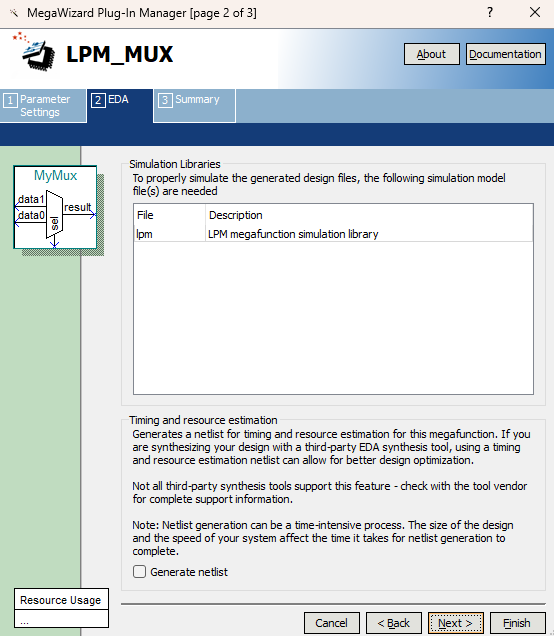
\includegraphics[scale=0.6]{IPCatalog4.png}
	\caption{Instanciación del multiplexor con \textit{IP Catalog} (Paso 4). \label{fig:ipcatalog4}}
\end{figure}

\begin{figure}[ht]
	\centering
	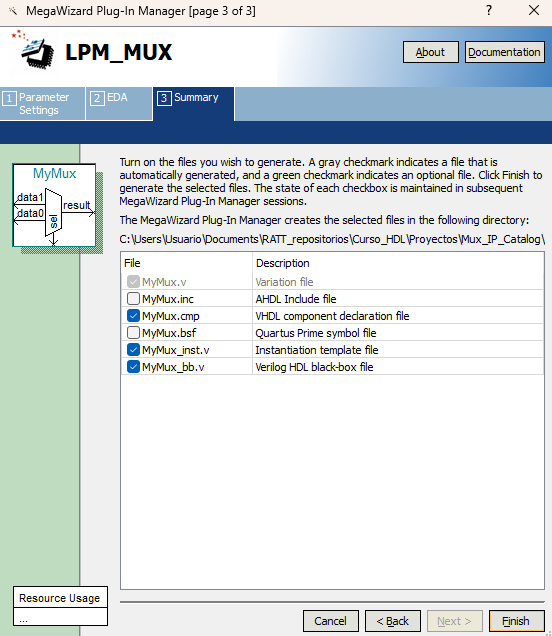
\includegraphics[scale=0.6]{IPCatalog5.png}
	\caption{Instanciación del multiplexor con \textit{IP Catalog} (Paso 5). \label{fig:ipcatalog5}}
\end{figure}

\begin{figure}[ht]
	\centering
	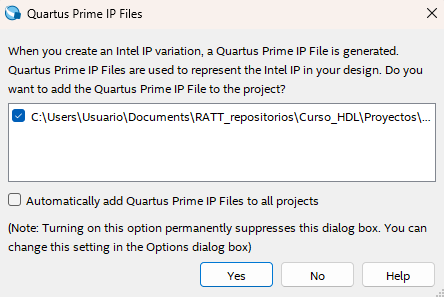
\includegraphics[scale=0.7]{IPCatalog6.png}
	\caption{Instanciación del multiplexor con \textit{IP Catalog} (Paso 6). \label{fig:ipcatalog6}}
\end{figure}

\begin{figure}[ht]
	\centering
	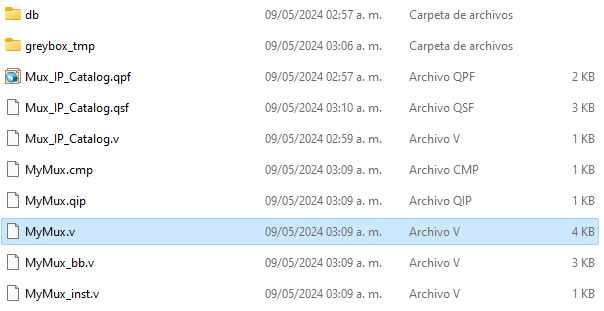
\includegraphics[scale=0.8]{IPCatalog7.png}
	\caption{Instanciación del multiplexor con \textit{IP Catalog} (Paso 7). \label{fig:ipcatalog7}}
\end{figure}

\begin{figure}[ht]
	\centering
	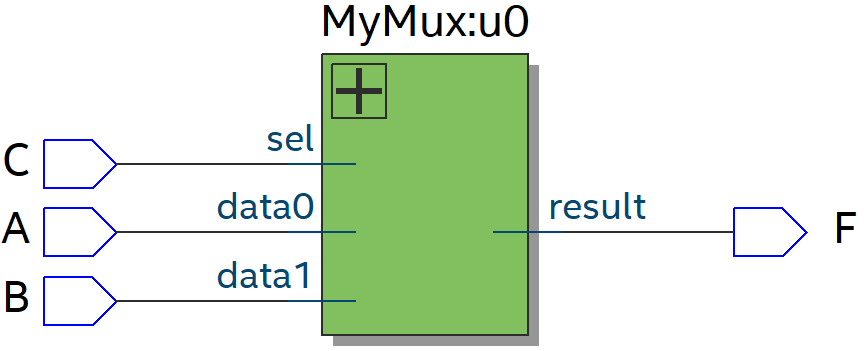
\includegraphics[scale=0.7]{Mux_IP_Catalog_RTL.png}
	\caption{Diagrama RTL del multiplexor, descrito en forma estructural con \textit{IP Catalog}. \label{fig:mux_ipcatalog_rtl}}
\end{figure}

\begin{figure}[ht]
	\centering
	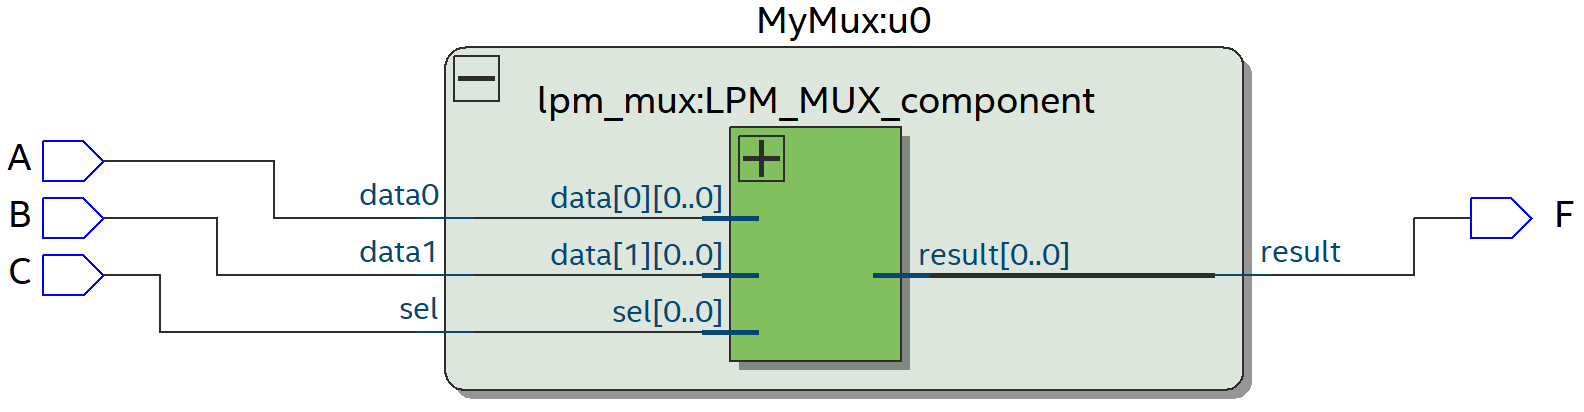
\includegraphics[scale=0.4]{Mux_IP_Catalog_RTL2.png}
	\caption{Diagrama RTL del multiplexor, descrito en forma estructural con \textit{IP Catalog} (visualización de la primera instancia interna). \label{fig:mux_ipcatalog_rtl2}}
\end{figure}

\begin{figure}[ht]
	\centering
	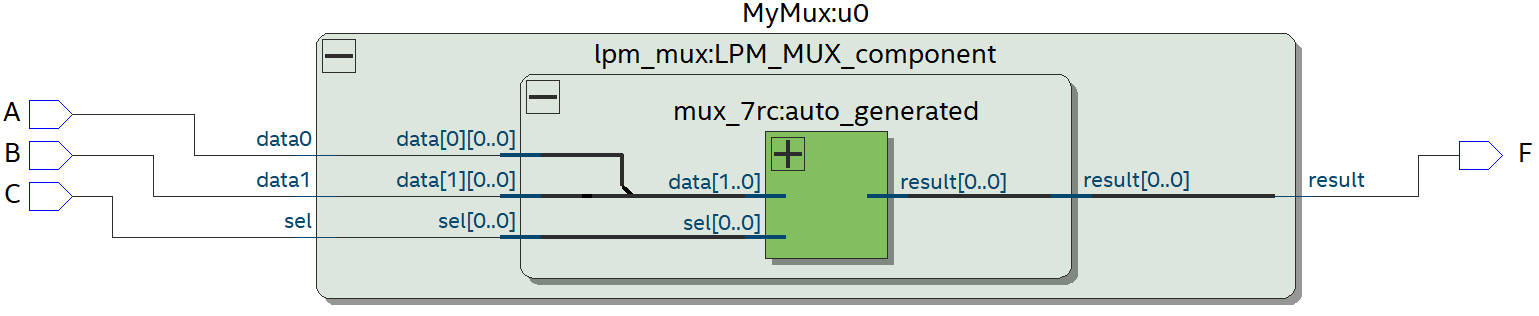
\includegraphics[scale=0.41]{Mux_IP_Catalog_RTL3.png}
	\caption{Diagrama RTL del multiplexor, descrito en forma estructural con \textit{IP Catalog} (visualización de la segunda instancia interna). \label{fig:mux_ipcatalog_rtl3}}
\end{figure}

\begin{figure}[ht]
	\centering
	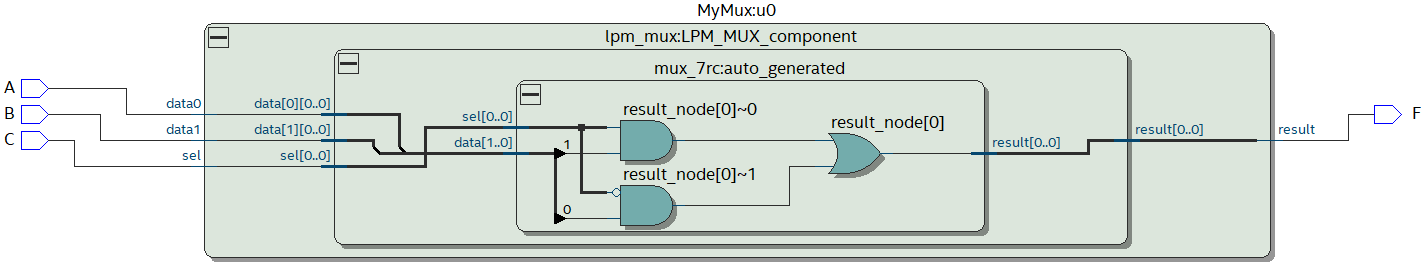
\includegraphics[scale=0.44]{Mux_IP_Catalog_RTL4.png}
	\caption{Diagrama RTL del multiplexor, descrito en forma estructural con \textit{IP Catalog} (visualización de la tercera instancia interna). \label{fig:mux_ipcatalog_rtl4}}
\end{figure}

\begin{figure}[ht]
	\centering
	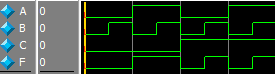
\includegraphics[scale=2]{Mux_IP_Catalog_Wave.png}
	\caption{Simulación del multiplexor, descrito en forma estructural con \textit{IP Catalog} en Verilog, con el visor de formas de onda de ModelSim. \label{fig:mux_ipcatalog_wave}}
\end{figure}